\documentclass[10pt]{article}
\usepackage[usenames]{color} %used for font color
\usepackage{amssymb} %maths
\usepackage{amsmath} %maths
\usepackage[utf8]{inputenc} %useful to type directly diacritic characters
\usepackage[letterpaper, portrait, margin=1.5in]{geometry}
\usepackage{graphicx,wrapfig}
\begin{document}
\subsection*{MSDS600 Week 8 Assignment - Nathan Worsham}
\subsection*{Step 1: Introduction to Hadoop Commands and experiments with the Hadoop commands }
Last week through trial and error I ended up learning about the hadoop file system in order to get my streaming example to work. There I learned that the HDFS is separate from the OS file system. So running through the file system commands this time felt more like a refresher.
\begin{wrapfigure}{r}{7cm}
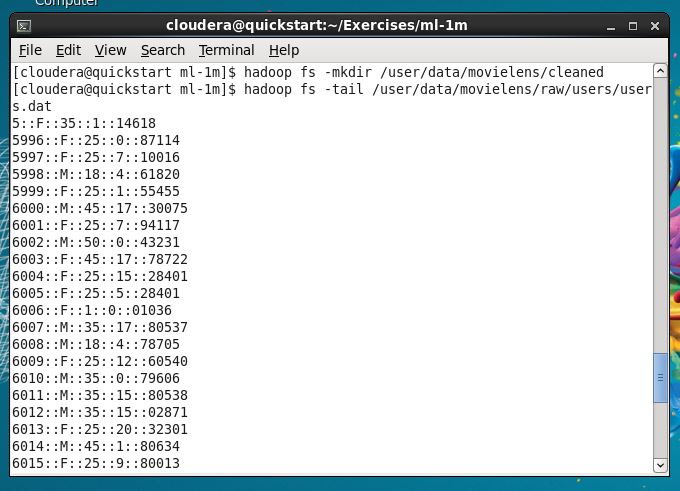
\includegraphics[width=7.5cm, scale=0.45]{week8_tail.jpg}
\end{wrapfigure}
\par I created the directories needed, put data in them, and confirmed the data. In the exercise it talks about tailing or cat -ing the file but in large files this is not good practice. I actually had an experience with this just recently where I had a folder that had grown accidentally to having 2.5 million files in it. Just doing a simple \verb|ls| of the directory is not something the OS can really even handle well, in fact even deleting them individually presents problems. In this case I removed the parent directory as a work around, but this is the reason that large file systems like HDFS and GFS exist.  

\subsection*{Step 2: Preprocessing data using Python}
I started the creation of my python scripts with trying to recreate the \verb|clean_ratings_dat.py|. The way I made my scripts differently is that I am used to coding Python in modules, so my scripts are made into functions and then the final main function brings everything together. This is considered the "pythonic way" and I find this is easier to troubleshoot large scripts because instead of having to comment out say 50 lines, you just comment out the one line that calls the function. When I was finished writing the script I tested it’s output against the example scripts output by running the original (my working directory was the scripts directory): 
\begin{verbatim}head ../ml-1m/ratings.dat|./clean_ratings.dat\end{verbatim}
and then comparing that output with my own: 
\begin{verbatim}head ../ml-1m/ratings.dat|./clean_ratings_myown.dat\end{verbatim}
The problem I found here was that my script was giving an an extra blank line in-between each output whereas the original was not. I realized the original had a \verb|line = line.strip()| which removes newline characters, so after adding this line of code my output then matched the example output.
\begin{figure}[!h]
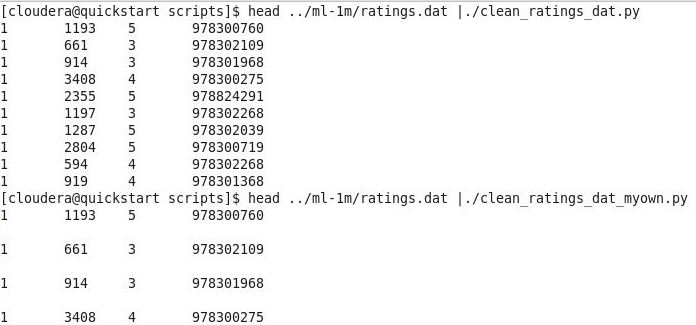
\includegraphics[scale=0.37]{missing_linestrip.jpg}
\centering
\end{figure}
\pagebreak
\par For the \verb|clean_movies_dat.py|, I only borrowed one section from the original which was the dictionary to convert the genres to the correct number. I then wrote my script made of three functions—one for converting genre to a number, one for pulling out the year using regex, and one to pull it all together. For my regex, I chose to be more specific than using \verb|.*| as I have been bitten by that in the past—the star quantifier is considered “greedy”(regular-expressions.info, n.d.). I instead elected to just look for the open and close parenthesis and look specifically for four digits--\verb|\(\d{4}\)|. Again running the example script first to compare output, I realized I had a syntax error, which after correcting that my output looked very similar except my list was printing out like a python list rather than a string. 
\begin{figure}[!h]
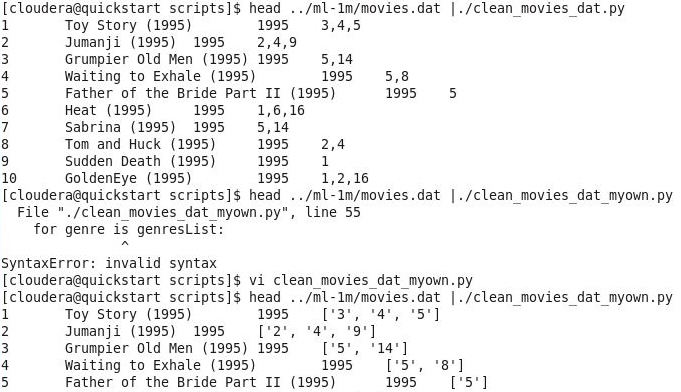
\includegraphics[scale=0.37]{clean_movies_error1.jpg}
\centering
\end{figure}\\
So I added a line 
\begin{verbatim}genresNumPrintList = ‘,’.join(genreNum)\end{verbatim}
and printed that instead. Now I had matching output.
\par For the final python script \verb|clean_users_dat.py|, I found that that running a test by increasing the number of lines to display from the file until I could find an example zip code with the -XXXX format (called delivery sector and segment) appended and then running this through the example script, that the appended dash and 4 digits were still in the data even though the requirements of the assignment said to do otherwise. Running it through my code I had planned to only present the first 5 digits of the zip code to correct this issue but I found that I had forgotten to specify that I wanted a range—I got an error because I put \verb|zipcode[5]| and indexes start with zero, so for many strings this character did not exist so I received the “index out of range” error. Correcting what I had meant to do I now found my code to work and successfully removed the extra zip code information.
\begin{figure}[!h]
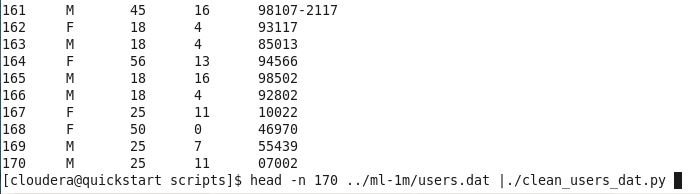
\includegraphics[scale=0.5]{broken_users_example.jpg}
\centering
\end{figure}
\begin{figure}[!h]
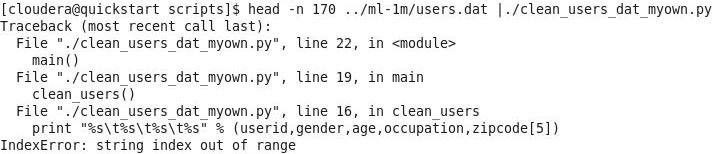
\includegraphics[scale=0.37]{clean_users_error1.jpg}
\centering
\end{figure}\\
\par For the bash script I really got my experience with the hadoop streaming command last week so interfacing with it was much better this go around. The one thing that threw me off at first was that there was no \verb|-reduce| option like there was in last weeks example but the assignment says to use the option \verb|-Dmapred.reduce.tasks=0| because the output of the mapper is the final output. Also the \verb|STREAMING| variable needed to be updated to run the correct jar (which is why it is good that it is set as a variable since it is subject to change). I successfully ran a mapreduce of each option—ratings, users, and movies. After each run, I would confirm the contents of the output directory with \verb|hadoop fs -ls directory| and then \verb|hadoop fs -tail| a specific file in the directory to confirm its contents.
\begin{figure}[!h]
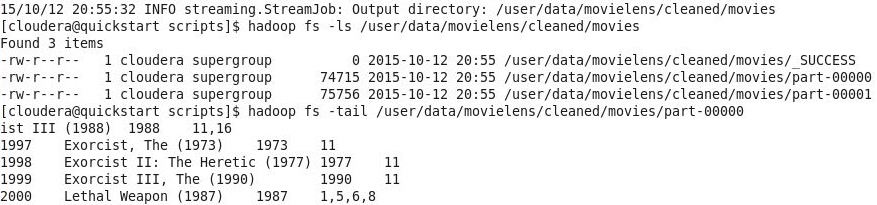
\includegraphics[scale=0.45]{mapreduce_movies_check.jpg}
\centering
\end{figure}
\subsection*{Step 3: Create Hive tables}
Following the HiveQL example, I queried \verb|select count(*) from users where age<35;| to answer the how many users under 35, I received a response of 3421. To answer who the top three users who rated the most, I ended up using Stackoverflow.com’s help. I was confused at first how to get this but by just looking at the data: \verb|select * from ratings limit 25;| I could see that really these were lines that could be counted by userid because each time a user rated a different movie it is written to a new row. So using the query 
\begin{verbatim}select userid,count(*) as count from ratings group by userid order by count
DESC limit 3;\end{verbatim}
I received this answer for the top three users who rated the most: 
\begin{verbatim}
4169    2314 
1680    1850 
4277    1743 
\end{verbatim}
With a total record of 1000209 ratings and 6040 users, these numbers seemed somewhat reasonable since 1000209/6040 is roughly 166, and you figure some users on rate once and some in the thousands. But I realized I could confirm this by querying a count of just my top user: \verb|select count(*) from ratings where userid=‘4169’;| and I received a match of 2314. After struggling with this question, the last question of how many users in each occupation I found to really be the same query as the second question because again I am just counting the number of rows by occupation. So using the query  
\begin{verbatim}
select occupation,count(*) as count from users group by occupation order by 
count DESC; 
\end{verbatim}
I received the answer of: 
\begin{figure}[!h]
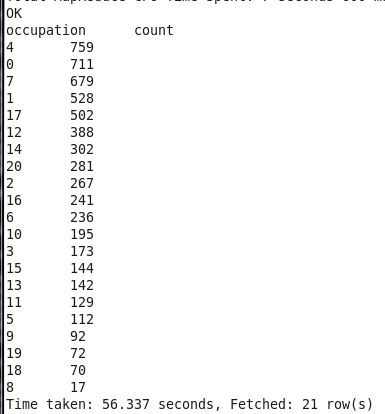
\includegraphics[scale=0.5]{occupation_query.jpg}
\centering
\end{figure}
\subsection*{Step 4: Build the basic recommender system using Mahout}
Running these scripts, I found again I needed to update the \verb|STREAMING| jar variable. I ran the map reduce command, tried to create the directory (already existed) and uploaded the user file. Next I was able to successfully run the \verb|do_mahout.sh| script. 
\begin{figure}[!h]
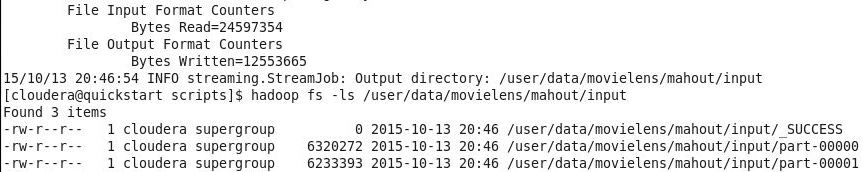
\includegraphics[scale=0.45]{mahout_mapreduce.jpg}
\centering
\end{figure}\\
Looking at the script, one thing I noticed was that it is set to use Pearson Correlation for its \verb|-similarityClassname| setting. Looking at the output, I noticed that it only returns recommendations for the user when it is predicting the user would rate the movie a 5. Taking user 1 as an example, 
\begin{verbatim}select * from ratings join movies on (ratings.movieid = movies.id) 
where ratings.userid=‘1’ and rating=‘5’;\end{verbatim} we see that some of the movies this user rated a 5 were “One Flew Over the Cuckoo’s Nest”, “Ben-Hur”, “A Bug’s Life”, and “Dog Park”.  Likewise grabbing a handful of the films that have been recommended, 
\begin{verbatim}select * from movies where id=‘1146’ or id=‘1012’ or id=‘1937’ or '2133’;\end{verbatim} The sample titles recommended: "Old Yeller", "Curtis's Charm", "Going My Way", and "Adventures in Babysitting". Now of course the user rated a lot more than I just gave as an example but are these good recommendations? I suppose you would have to ask user 1. Though from a critical acclaim point-of-view, the 4 movies I chose which user 1 rated are all highly rated on rottentomates.com (88-95\%) with the exception of "Dog Park", which only scores a 36\%. So user 1 (and probably everyone) clearly has some eclectic tastes.
\subsection*{References}
Decalage.info, n.d. Retrieved from http://www.decalage.info/en/python/print\_list\\
Soniak, Matt. 2013. Retrieved from http://mentalfloss.com/article/53384/what\%E2\%80\%99s-deal-those-last-4-digits-zip-codes\\
Stackoverflow.com, n.d. Retrieved from http://stackoverflow.com/questions/9994970/counting-in-hadoop-hive\\
Regular-expressions.info, n.d. Retrieved from http://www.regular-expressions.info/repeat.html\\
Rottentomatoes.com, n.d. Retrieved from http://www.rottentomatoes.com/m/dog\_park
\end{document}